\documentclass[10.5pt]{article}
\usepackage[T1]{fontenc}
\usepackage{titling}
\usepackage{enumitem}
\usepackage{xcolor}
\usepackage{cite}
\usepackage{amsmath, amsfonts, amssymb, amsthm,tikz}
\usepackage[a4paper, total={6.6in, 8.7in}]{geometry}
\usepackage{fancyhdr}
\usepackage{parskip}
\usepackage{float}
\usepackage{caption}
\usepackage{subcaption}
\usepackage{mathtools}
\usepackage{cancel}
\usepackage{verbatim} 
\setenumerate[1]{label=(\arabic*)}
\renewcommand{\qedsymbol}{$\blacksquare$}
\renewcommand{\implies}{\Rightarrow}
\newcommand\cc{\mathcal}
\newcommand\bb{\mathbb}
\newcommand\bbcdot{\boldsymbol{\cdot}}
\newcommand\inv[1]{#1^{-1}}
\newcommand\todo[1]{\color{red} \textbf{TODO: } #1 \color{black}}
\newcommand\hint[1]{\color{blue} \textit{HINT: #1} \color{black}}
\newcommand\cl{\overline}
\newcommand\D{\partial}
\DeclareMathOperator{\Tr}{Tr}
\DeclareMathOperator{\Id}{Id}
\DeclareMathOperator{\Sp}{span}
\DeclareMathOperator{\Ker}{Ker}
\DeclareMathOperator{\Ran}{Ran}
\DeclareMathOperator{\argmax}{argmax}
\DeclareMathOperator{\ImPart}{Im}
\DeclareMathOperator{\Span}{span}
\DeclareMathOperator{\RePart}{Re}
\DeclareMathOperator{\Arg}{Arg}
\DeclareMathOperator{\supp}{supp}
\DeclareMathOperator{\Image}{Image}
\pagestyle{fancy}
\fancyhf{}
\fancyhead[RO]{CBO+BFF applied to Q-control}
\fancyhead[LO]{Insulla, Zhu, Ying}
\fancyfoot[RO]{Page \thepage}
\renewcommand{\headrulewidth}{1pt}
\renewcommand{\footrulewidth}{1pt}
\setlength{\headheight}{13.6pt}
\newtheorem{lemma}{Lemma}
\newtheorem{theorem}{Theorem}
\setlength{\droptitle}{-10em}
\usepackage{lmodern}
\title{CBO + BFF applied to Q-control}
\author{Francesco Insulla, Yuhua Zhu, Lexing Ying}
\begin{document}
\maketitle

\section{Introduction}

Recently there has been progress in applying a novel gradient-free optimization heuristic to high dimensional machine learning, called Consensus Based Optimization (CBO) \cite{carrillo2020consensusbased}, and on a novel sampling method for Reinforcement Learning (RL), called Borrowing from Future (BFF) \cite{zhu2020borrowing}. Given the advantages CBO and BFF individually, we explore if there is an advantage to using both. We first introduce Bellman residual minimization (BRM) for Q-control and outline CBO vs Stochastic Gradient Descent (SGD) and BFF vs UR (Unrealistic) vs DS (Double) sampling. Next we prove some results for the difference between UR and BFF in CBO. We then setup a numerical example is continuous and discrete statespace, outline a procedure, and analyze the results. Finally, we give an upper bound on the difference in CBO's parameter modification using BFF vs UR. While CBO+BFF appears advantageous in the discrete case, this is not the case for the continuous case, likely attributable to the higher dimensionality of the hyperparameter space for CBO and/or the highly non-convex loss function for the continuous case.

\section{Models}

In $Q$-control, the objective is to find a $Q^*:\bb S\times \bb A\to \bb R$ satisfying the Bellman equation $Q^*(s,a)=\bb T^{\pi_*} Q^*(s,a)$ where
$$
\bb T^{\pi_*} Q^*(s,a) = \bb E\Big[r(s_{m+1},s_m, a_m)+\gamma \max_{a'}Q^*(s_{m+1},a';\theta)\Big|(s_m, a_m)=(s,a)\Big]
$$
One method of doing this is to solve the Bellman residual minimization (BRM) problem, which amounts to minimizing $J(\theta)=\bb E[\delta^2(s,a;\theta)]$ where $\delta(s,a;\theta) = \bb T^{\pi_*}Q^*(s,a) -Q^*(s,a)$, i.e.
\begin{align*}
    J(\theta) &= \mathbb E[((\mathbb T^{\pi_*}-\mathbb I) Q^*(s,a;\theta))^2]\\
&= \mathbb E[\mathbb E[j^{ctrl}(s_m, a_m, s_{m+1};\theta)|s_m,a_m]^2]\\
j^{\text{ctrl}}(s_m, a_m, s_{m+1};\theta) &= r(s_{m+1}, s_m, a_m)  + \gamma \max_{a'} Q^*(s_{m+1},a';\theta) - Q^*(s_m,a_m;\theta)
\end{align*}

Solving this minimization problem requires an optimization scheme and a sampling method.

For the optimization schemes, we consider Stochastic Gradient Descent (SGD) and Consensus Based Optimization (CBO).

At iteration $k$, with batch $B_k$, samples $\{(s_m, a_m, s_{m+1},s_{m+1}')\}_{m\in B_k}$, parameters $\theta_k$, and learning rate $\tau_k$, SGD is formulated by the following update equation

\begin{align*}
  \hat F_k &= \frac{1}{|B_k|}\sum_{m\in B_k} j^{\text{ctrl}}(s_m, a_m, s_{m+1};\theta_k )\nabla_\theta j^{\text{ctrl}}(s_m, a_m, s_{m+1}';\theta_k)\\
  \Delta\theta_k &= -\tau_k \hat F_k 
\end{align*}

At iteration $k$, with batch $B_k$, samples $\{(s_m, a_m, s_{m+1},s_{m+1}')\}_{m\in B_k}$, particle parameters $\{\theta_k\}_{j=1}^N$, learning rate $\eta_k$, diffusion rate $\tau_k$, and inverse temperature $\beta_k$, CBO is formulated by the following update equation

\begin{align*}
  \hat J_k^j &= \frac{1}{|B_k|}\sum_{m\in B_k} j^{\text{ctrl}}(s_m, a_m, s_{m+1};\theta_{k}^j) j^{\text{ctrl}}(s_m, a_m, \tilde s_{m+1};\theta_{k}^j)\\
  \bar\theta_k &= \frac{\sum_{j=1}^N \theta^{j}_{k} e^{-\beta_k \hat J^j_k}}{\sum_{j=1}^N  e^{-\beta_k\hat J_k^j}}\\
  \Delta \theta^{j}_k &= (-\eta_k \lambda_k I+\tau_k\sqrt{\eta_k} Z_j)(\theta^j_{k}-\bar\theta_k); \quad Z_j\sim \text{diag}(\mathcal N(0,I))
\end{align*}
additionally, the CBO algorithm checks if $\|\Delta \theta^j_k\|<\delta$ and adds $\tau_k \sqrt \eta_k Z_j'$ to $\Delta \theta_k^j$, with $Z_j'\sim\text{diag}(\mathcal N(0,I))$.

Given $(s_m,a_m,s_{m+1})$ we need a sampling method to generate $\tilde s_{m+1}$, ideally from the dynamics of the model which are unknown. Assume the dynamics of the model have the form
$$\Delta s_m = \mu(s_m, a_m) \epsilon + \sigma_m \sqrt \epsilon z_m$$ with $a_m\sim \pi_b(\cdot|s_m)$ and $z_m\sim \cc N(0,I)$. Unrealistic sampling (UR/Uncorrelated Sampling) generates $\tilde s_{m+1}$ directly from the dynamics of the model, Double Sampling (DS/Sample Cloning) reuses the original sample setting $\tilde s_{m+1}=s_{m+1}$, and Borrowing From the Future (BFF) exploits a difference with a future sample setting $\tilde s_{m+1}=s_m+\Delta s_{m+1}$ where $\Delta s_{m+1}=s_{m+2}-s_{m+1}$.

\section{Theoretical Results}
\subsection{Difference in UR vs BFF in CBO}
We consider the CBO model with UR and BFF sampling and prove resulting relating to convergence. The approach is adapted from \cite{zhu2020borrowing}, where a similar analysis is done for SGD.

Taking $N\to \infty$, $\eta\to 0$, the mean field limit of CBO model is given by the following SDE with corresponding Fokker-Planck equation
\begin{align*}
  d\Theta &= -\lambda(\Theta - \bar \Theta)dt + \tau \sum_{i=1}^d e^{(i)} (\Theta - \bar \Theta)_i dW_i \\
  \bar \Theta &= \frac{\bb E_\Theta[ \Theta e^{-\beta J(\Theta)} ]}{\bb E_\Theta[e^{-\beta J(\Theta)}]}\\
  \partial_t \rho &= \lambda \nabla \cdot ((\Theta - \bar \Theta) \rho ) + \frac{1}{2}\tau^2 \sum_{i=1}^d\partial_{ii}((\Theta - \bar \Theta)_i \rho)
\end{align*}
Where $\Theta_{k}\approx \theta_{\eta k}$.
As $\bar \Theta$ depends on the sample $s,a$, we approximate the process as
\begin{align*}
  d\Theta &= -\lambda (\Theta - \bb E_{s,a}[\bar \Theta])dt + \tau \sum_{i=1}^d e^{(i)} (\Theta - \bb E_{s,a}[\bar \Theta])_i dW_i + \lambda \eta^{1/2}\, \bb V_{s,a}[\bar\Theta]^{1/2}  dW_0\\
  \partial_t \rho &= \lambda \nabla \cdot ((\Theta - \bb E_{s,a}[\bar \Theta]) \rho ) + \frac{1}{2} \sum_{i=1}^d\partial_{ii}((\tau^2(\Theta - \bb E_{s,a}[\bar \Theta])^2_i+\lambda^2\eta \bb V_{s,a}[\bar \Theta]_{ii} ) \rho)
\end{align*}
% \begin{align*}
%   d\Theta &= -\lambda \bb E_{s,a}[\Theta - \bar \Theta]dt + \tau \sum_{i=1}^d e^{(i)} \bb E_{s,a}[(\Theta - \bar \Theta)_i^2]^{1/2} dW_i \\
%   \partial_t \rho &= \lambda \nabla \cdot (\bb E_{s,a}[\Theta - \bar \Theta] \rho ) + \frac{1}{2}\tau^2 \sum_{i=1}^d\partial_{ii}(\bb E_{s,a}[(\Theta - \bar \Theta)_{i}^2] \rho)
% \end{align*}

We leave the proof of that the approximation is correct for future study. Intuitively, similarly to how SGD is approximated, $\bar \Theta = \bb E_{s,a}[\bar \Theta] + \eta^{1/2}\bb V_{s,a}[\bar \Theta]^{1/2}\frac{dW_0}{dt}$.
Henceforth, we use $\delta$ denote any difference between a UR and BFF quantity, such as $\delta J(\Theta)= J(s,\Theta) - J(s',\Theta)$.

\begin{lemma}
  Fix $t$. Assume
  $\sup_{s\in \bb S,a\in \bb A}|\bb E_a[\mu(s,a)|s] - \mu(s,a)| \leq  v$,
  $\sup_{s\in \bb S}\| \bar \Theta(s)\| \leq  m$,
  $\sup_{s\in \bb S}\|\partial_s \bar \Theta(s)\| \leq m_s$.
  % \begin{align*}
  % &\sup_{s\in \bb S,a\in \bb A}|\bb E[\mu(s,a)|s] - \mu(s,a)| \leq  v,\\
  % &\sup_{s\in \bb S}\|\bar \Theta(s)\| \leq  m,\\
  % &\sup_{s\in \bb S}\|\partial_s \bar \Theta(s)\| \leq m_s
  % \end{align*}
  almost surely.
  Then
  % \begin{align*}
  %   |\delta \bb E[\bar \Theta]| &\leq \epsilon C |\bb E[\partial_s \bar \Theta(s_m)]| + O(\epsilon^2)\\
  %   |\delta \bb V[\bar \Theta(\tilde s_{m+1})]| &\leq 2 \epsilon C\bb C[\bar \Theta(s_m), \partial_s \bar \Theta(s_m)]+ O(\epsilon^2)
  % \end{align*}
  \begin{align*}
    \|\delta \bb E_{s,a}[\bar \Theta]\| &\leq \epsilon v m_s + o(\epsilon)\\
    % |\delta \bb V[\bar \Theta(\tilde s_{m+1})]| &\leq 2 \epsilon v u u_s + O(\epsilon^2)\\
    % \|\delta \bb E_{s,a}[(\Theta - \bar \Theta)_i^2]\| &\leq 2 \epsilon v m m_s + O(\epsilon^2)
    |\delta (\Theta - \bb E_{s,a}[\bar \Theta])_i^2| &\leq \epsilon v m m_s + o(\epsilon)
  \end{align*}

  % \color{red}
  % Let $\|\bb E[a|s]\|_\infty=u$, $\|\nabla_s \bb E[a|s]\|_\infty = u_s$ and $\|a - \bb E[a|s]\|_\infty  = v $ and assume $u,u_s,v<\infty$.

  % \color{blue}
  % Let $C = \|j(s,\theta)\|_\infty,$$C_s = \|\nabla_s j(s,\theta)\|_\infty,$$C_\theta = \|\nabla_\theta j(s,\theta)\|_\infty,$$C_{s,\theta} = \|\nabla_s\nabla_\theta j(s,\theta)\|_\infty$ and assume $C,C_s,C_\theta,C_{s,\theta}<\infty$.


  % \color{red}
  % Let $f(s,\theta) = \max_{a\in \bb A} Q^*(s,a,\theta)$ and $g(\theta)=Q^*(\theta)$. Let $\|\partial_s r(s) + \partial_s f(s,\theta)\|_\infty = C_s$, $\|\nabla_\theta g\|_\infty = C_\theta$, $\|\partial_s\nabla_\theta f(s,\theta)\|_\infty =C_{s,\theta}$ and assume $C_s,C_\theta,C_{s,\theta} < \infty$. Assume $\|j(s,\theta)^2\|_\infty < \infty$.

  % Assume that
  % \begin{align*}
  %   \bb E[e^{(\alpha\epsilon/r)^2 \| a - \bb E[a|s]\|^2}|s]
  % \end{align*}
  % and $\|\bb E[a|s] - \bb E[a|s']\|^2 \leq C_{a,s}^2\|s-s'\|^2 $ for some $0<C_a,C_{a,s}<\infty$. Assume also that there exists $w,\nu$ such that, 
  % \begin{align*}
  %   \int
  %   d\Theta\,d\Phi \rho(\Theta) \rho(\Phi)
  %   e^{\lambda \|\Theta - \Phi\|^2} \leq e^{\lambda w^2}
  % \end{align*}
  % for all $\lambda > 0$, and
  % \begin{align*}
  %   1-4\beta^2(\|j(s,\theta)^2\|_\infty C_{s,\theta}^2 + C_s^2 C_\theta^2)w^2 \epsilon = r^2 >  0
  % \end{align*}
  % Then \color{red}
  % \begin{align*}
  % |\delta \bb E[ \bar\Theta   ]| &\leq\\
  % |\delta \bb V[ \bar \Theta_i ]| &\leq
  % \end{align*}
\end{lemma}
\begin{proof}
  Taylor expanding $\bar \Theta(\tilde s)$ about $s_m$ we find 
  \begin{align*}
    \bar \Theta(\tilde s_{m+1}) &= \bar \Theta(s_m) + (\tilde s_{m+1} - s_m)\partial_s \bar \Theta(s_m) + \tfrac{1}{2}(\tilde s_{m+1} - s_m)^2\partial^2_s \bar \Theta(s_m) + o(\epsilon)
  \end{align*}
  Note that
  \begin{align*}
    \tilde s_{m+1} - s_m &= \mu(s_m, a_m)\epsilon + \sigma\epsilon^{1/2} Z_m\\
    \tilde s_{m+1}' - s_m &= \mu(s_m, a_{m+1})\epsilon + \sigma\epsilon^{1/2} Z_{m+1}
  \end{align*}
  Thus
  \begin{align*}
    \bb E[\bar \Theta(\tilde s_{m+1})|a_m,s_m] &= \bar \Theta(s_m) - \epsilon \mu(s_m,a_m)\partial_s \bar \Theta(s_m) + \tfrac{1}{2}(\sigma^2 \epsilon) \partial^2_s \bar \Theta(s_m) + o(\epsilon)\\
    \bb E[\bar \Theta(\tilde s_{m+1}')|a_m,s_m] &= \bar \Theta(s_m) - \epsilon \bb E[\mu(s_m,a_{m+1})|s_m]\partial_s \bar \Theta(s_m) + \tfrac{1}{2}(\sigma^2 \epsilon) \partial^2_s \bar \Theta(s_m) + o(\epsilon)\\
    \delta \bb E[ \bar \Theta |a_m,s_m] &= \epsilon(\bb E[\mu(s_m,a_{m+1})|s_m]-\mu(s_m,a_m))\partial_s \bar \Theta(s_m) + o(\epsilon)
  \end{align*}
  Taylor expanding $\pi(a|s)$ about $s_{m+1}$ we have
  \begin{align*}
    \bb E[\mu(s_m,a_{m+1})|s_m] 
    &=  \int da\, \mu(s_m, a) \pi(a|s_{m+1})\\
    &=  \int da\, \mu(s_m, a) (\pi(a|s_m)+\partial_s \pi(a|s_m)(\mu(s_m,a_m)\epsilon + \sigma\epsilon^{1/2}Z_m)) + O(\epsilon)\\
    &= \bb E[\mu(s_m,a_m)|s_m] + O(\epsilon^{1/2})
  \end{align*}
  Thus
  \begin{align*}
    \|\delta \bb E_{s,a}[\bar \Theta]\| \leq \epsilon v m_s + o(\epsilon)
  \end{align*}
  Similarly we find
  % \begin{align*}
  %   \bb V[\bar \Theta(\tilde s_{m+1})|a_m,s_m] &= 
  %   \sigma^2\epsilon(\partial_s \bar \Theta(s_m))^2 + 
  %   2\sigma^4\epsilon^2 (\partial_s^2 \bar \Theta(s_m))^2 + 
  %   o(\epsilon^2)\\
  %   \bb V[\bar \Theta(\tilde s_{m+1}')|a_m,s_m] &= 
  %   (\epsilon^2 \bb V[\mu(s_m, a_{m+1})|s_m]+ \sigma^2\epsilon )(\partial_s \bar \Theta(s_m))^2+
  %   2\sigma^4\epsilon^2 (\partial_s^2 \bar \Theta(s_m))^2 + 
  %   o(\epsilon^2)
  %   % \delta \bb V[\bar \Theta|a_m,  s_m] &= \epsilon^2 \bb V[\mu(s_m, a_{m+1})|s_m] (\partial_s \bar \Theta(s_m))^2 + o(\epsilon^2)
  % \end{align*}
  % Using the previous result,
  % \begin{align*}
  %   \delta \bb V[\bar \Theta(\tilde s_{m+1})] 
  %   &= \delta \bb V[\bb E[\bar \Theta(\tilde s_{m+1})|s_m,a_m]
  %   + \delta \bb E[\bb V[\bar \Theta(\tilde s_{m+1})|s_m,a_m]\\
  %   \delta \bb E[\bb V[\bar \Theta(\tilde s_{m+1})|s_m,a_m] 
  %   &= O(\epsilon^2)\\
  %   \delta \bb V[\bb E[\bar \Theta(\tilde s_{m+1})|s_m,a_m]
  %   &= 2\epsilon (\bb C[\bar \Theta(s_m),  \mu(s_m,a_m)\partial_s \bar \Theta(s_m)]-\bb C[\bar \Theta(s_m),  \bb E[\mu(s_m,a_{m+1})|s_m]\partial_s \bar \Theta(s_m)]) + O(\epsilon^2)\\
  %   &= 2\epsilon \bb E[\mu(s_m,a_m) - \bb E[\mu(s_m,a_{m+1})|s_m]]\bb C[\bar \Theta(s_m), \partial_s \bar \Theta(s_m)]+ O(\epsilon^2)
  % \end{align*}
  % And
  \begin{align*}
    \delta \bb E[ (\Theta - \bar \Theta)_i |a_m,s_m]^2 = \epsilon(\Theta - \bar \Theta(s_m))_i (\bb E[\mu(s_m,a_{m+1})|s_m]-\mu(s_m,a_m))\partial_s \bar \Theta_i(s_m) + O(\epsilon^2)
  \end{align*}
  Thus
  \begin{align*}
    % \delta \bb E_{s,a}[(\Theta - \bar \Theta(\tilde s_{m+1}))_i^2]\| &\leq 3 \epsilon v m m_s + O(\epsilon^2)
    |\delta (\Theta - \bb E_{s,a}[\bar \Theta])_i^2| &\leq \epsilon v m m_s + o(\epsilon)
  \end{align*}
\end{proof}
  % \begin{lemma}
  %   Assume ....

  %   Then
  %   \begin{align*}
  %     \bb E[\partial_s \bar \Theta(s)] & \\
  %     \bb C[\bar \Theta(s), \partial_s \bar \Theta(s)] &
  %   \end{align*}
  % \end{lemma}
  % \begin{proof}
  %   Let $H_{s,\beta}(\Theta) = -\log \rho(\Theta) + \beta J(s,\Theta)$, $\tilde \rho_{s,\beta}(\Theta) = Z_{s,\beta}^{-1} e^{-H_{s,\beta}(\Theta)}$, $\tilde{\bb E}_{s,\beta} $ be the expectation over $\Theta \sim \tilde \rho_{s,\beta}$, and $\bar \Theta_\beta(s) = \tilde{\bb E}_{s,\beta}[\Theta]$.

  %   Then
  %   \begin{align*}
  %     \partial_s \bar \Theta_\beta(s)
  %     &= -\tilde{\bb E}_{s,\beta}[(\Theta - \tilde{\bb E}_{s,\beta}[\Theta])(\beta \partial_s J(s,\Theta) - \tilde{\bb E}_{s,\beta}[\beta\partial_s  J(s,\Theta)])]\\
  %     &= -\tilde{\bb C}_{s,\beta}[\Theta,\beta \partial_s J(s,\Theta)]\\
  %     \|\partial_s \bar \Theta(s)\|^2 &\leq \Tr \tilde{\bb V}_{s,\beta}[\Theta ]\tilde{\bb V}_{s,\beta}[\beta\partial_s  J(s,\Theta)]
  %   \end{align*}

  %   % Taylor expanding $H_{s,\beta}(\Theta) $ about its minimum $\hat \Theta_{s,\beta}$ (i.e. the mode of $\rho_{s,\beta}$) we get
  %   % \begin{align*}
  %   %   H_{s,\beta} (\Theta) =&
  %   %   H_{s,\beta}(\hat \Theta_{s,0})
  %   %   % + (\Theta - \hat \Theta_{s,\beta})\nabla_\Theta H_{s,\beta}(\hat \Theta_{s,\beta})\\
  %   %   + \tfrac{1}{2}(\Theta - \hat \Theta_{s,\beta})^T \nabla_\Theta \nabla_\Theta^T H_{s,\beta}(\hat \Theta_{s,\beta})(\Theta - \hat \Theta_{s,\beta}) + o(\|\Theta - \hat \Theta_{s,\beta}\|^2)
  %   % \end{align*}

  %   % Thus
  %   % \begin{align*}
  %   %   \tilde{\bb V}_{s,\beta}[\Theta]  \approx \inv{(\nabla_\Theta \nabla_\Theta^T H_{s,\beta}(\bar \Theta_{s,\beta}))} = \inv{(\nabla_\Theta \nabla_\Theta^T H_{0}(\bar \Theta_{s,\beta}) + \beta \nabla_\Theta \nabla_\Theta^T J(s,\bar \Theta_{s,\beta}))}
  %   % \end{align*}
  % \end{proof}
  % \color{blue}

  % \begin{align*}
  %   \delta \bb V[\bar \Theta(\tilde s_{m+1})]
  %   =& \delta \bb V[\bb E[\bar \Theta(\tilde s_{m+1})|s_m,a_m]
  %   + \delta \bb E[\bb V[\bar \Theta(\tilde s_{m+1})|s_m,a_m]\\
  %   \delta \bb E[\bb V[\bar \Theta(\tilde s_{m+1})|s_m,a_m]
  %   =& -\epsilon^2 \bb E[\bb V[\mu(s_m, a_{m+1})|s_m]]\bb E[(\partial_s \bar \Theta(s_m))^2]+o(\epsilon^2)\\
  %   \delta \bb V[\bb E[\bar \Theta(\tilde s_{m+1})|s_m,a_m]
  %   =&
  %   2\epsilon (\bb C[\bar \Theta(s_m),  \mu(s_m,a_m)\partial_s \bar \Theta(s_m)]-\bb C[\bar \Theta(s_m),  \bb E[\mu(s_m,a_{m+1})|s_m]\partial_s \bar \Theta(s_m)])\\
  %   &+\epsilon^2 (\bb V[\mu(s_m,a_m)\partial_s \bar \Theta(s_m)] - \bb V[\bb E[\mu(s_m,a_{m+1})|s_m]\partial_s \bar \Theta(s_m)])\\
  %   &+\epsilon^2 \sigma^2(\bb C[\mu(s_m,a_m)\partial_s\bar \Theta(s_m),\partial_s^2\bar \Theta(s_m)] -
  %   \bb C[\bb E[\mu(s_m,a_{m+1})|s_m]\partial_s\bar \Theta(s_m),\partial_s^2\bar \Theta(s_m)])\\
  %   &+o(\epsilon^2)\\
  %   =&
  %   2\epsilon \bb E[\mu(s_m,a_m) - \bb E[\mu(s_m,a_{m+1})|s_m]]\bb C[\bar \Theta(s_m), \partial_s \bar \Theta(s_m)]\\
  %   &+\epsilon^2 (\bb E[\mu(s_m,a_m)^2]-\bb E[\bb E[\mu(s_m,a_{m+1})|s_m]^2])\bb V[\partial_s \bar \Theta(s_m)]\\
  %   &+\epsilon^2 (\bb V[\mu(s_m,a_m)]-\bb V[\bb E[\mu(s_m,a_{m+1})|s_m]])\bb E[\partial_s \bar \Theta(s_m)]^2\\
  %   &+\epsilon^2 \sigma^2\bb E[\mu(s_m,a_m) -\bb E[\mu(s_m,a_{m+1})|s_m]]\bb C[\partial_s\bar \Theta(s_m),\partial_s^2\bar \Theta(s_m)]\\
  %   &+o(\epsilon^2)\\
  % \end{align*}
%   \color{purple}

%   We Taylor expand $\Theta$, take the $\delta$ difference, evaluate and bound to get
%   % Let $\tilde \rho_{ s}(\Theta) = \inv{Z( s)} \rho(\Theta)e^{-\beta J( s,\Theta) }$ and $\tilde{\bb E}_{ s}$ be the expectation over $\Theta \sim \tilde \rho_{ s}$.
%   % Then $\bar \Theta( s) = \tilde {\bb E}_{ s}[\Theta]$
%   \begin{align*}
%     \bar \Theta(\tilde s_{m+1}) &= \bar \Theta(s_m) + (\tilde s_{m+1} - s_m)\partial_s \bar \Theta(s_m) + \tfrac{1}{2}(\tilde s_{m+1} - s_m)^2\partial^2_s \bar \Theta(s_m) + o(\epsilon)\\
%     \delta\bar \Theta &=  \delta(\tilde s_{m+1} - s_m)\partial_s \bar \Theta(s_m) + \tfrac{1}{2}\delta((\tilde s_{m+1} - s_m)^2)\partial^2_s \bar \Theta(s_m) + o(\epsilon)\\
%     \bb E[\delta(\tilde s_{m+1} - s_m)|s_m,s_{m+1} ] &= (\bb E[a_{m}|s_m] - \bb E[a_{m+1}|s_{m+1}])\epsilon\\
%     \bb E[\delta((\tilde s_{m+1} - s_m)^2)|s_m,s_{m+1} ] &= (\bb E[a_{m}^2|s_m] - \bb E[a_{m+1}^2|s_{m+1}])\epsilon^2 = o(\epsilon)\\
%     |\delta \bar \Theta| &\leq u_s \epsilon \|\partial_s \bar \Theta\|_\infty  + o(\epsilon)
%     % \delta \bb E[\bar \Theta]
%     % &= \bb E[\delta \bar \Theta]\\
%     % \delta\bar\Theta
%     % &= \bar \Theta(\tilde s) - \bar \Theta(\tilde s')\\
%     % &= \bar \Theta(\tilde s) - \bar \Theta(\tilde s - \delta \tilde s)\\
%     % &= \partial_s \bar \Theta(s) \delta \tilde s - \tfrac{1}{2}\partial^2_s \bar \Theta(s) (\delta \tilde s)^2 + o(\epsilon)
%     % |\delta \bar \Theta| &\leq |\delta \tilde s| \|\partial_s\bar \Theta(s)\|_\infty
%   \end{align*}

%   Next, note that 
%   \begin{align*}
%     \bb E[|\delta \tilde s|^2]
%     &= \bb E[|\tilde a_m - a_{m+1}|^2]\epsilon^2 + 2\sigma^2 \epsilon\\
%     |\tilde a_m -  a_{m+1}|^2
%     &= |\tilde a_m - \bb E[a_m|s_m]|^2 + | a_{m+1} - \bb E[a_{m+1}|s_{m+1}]|^2  + | \bb E[a_m|s_m] - \bb E[a_{m+1}|s_{m+1}]|^2 \\
%     &\leq 2v^2+ u_s^2|s_m - s_{m+1}|^2\\
%     \bb E[|s_m - s_{m+1}|^2]
%     &\leq \epsilon^2(v^2+u^2)+ \sigma^2\epsilon\\
%     \bb E[|\delta \tilde s|^2] 
%     % &\leq \epsilon^2(2v^2 + u_s^2(\epsilon^2(v^2+u^2)+ \sigma^2\epsilon)) + 2\sigma^2\epsilon
%     &\leq \epsilon(2\sigma^2) + \epsilon^2(2v^2)+\epsilon^3(\sigma^2)+\epsilon^4(u_s^2(v^2+u^2))=O(\epsilon)
%   \end{align*}


%   Note that
%   \begin{align*}
%     \partial_s \bar \Theta(s) &= -\tilde{\bb E}_s[(\Theta - \tilde{\bb E}_s[\Theta])(\beta \partial_s J(s,\Theta) - \tilde{\bb E}_s[\beta\partial_s  J(s,\Theta)])]\\
%     &= -\tilde{\bb C}_s[\Theta,\beta \partial_s J(s,\Theta)]\\
%     |\partial_s \bar \Theta_i(s)|^2 &\leq \tilde{\bb V}_s[\Theta_i ]\tilde{\bb V}_s[\beta\partial_s  J(s,\Theta)]
%   \end{align*}







% % \begin{comment}
%   \color{red}
%   % Let $\tilde \rho_{\beta, J} (\Theta) = Z^{-1}_{\beta,J} e^{-\beta J(\Theta)}$.
%   First, we express $\delta \bar \Theta$ more conveniently as
%   \begin{align*}
%     \delta \bar\Theta
%     &=\frac{\tfrac{1}{2}\int d\Theta\, d\Theta'\, \rho(\Theta)\rho(\Theta')(\Theta - \Theta') (e^{-\beta(J(\Theta)+ J'(\Theta'))}- e^{-\beta(J'(\Theta)+ J(\Theta'))} )}{\int d\Theta\,d\Theta' \,  \rho(\Theta)\rho(\Theta') e^{-\beta(J(\Theta)+ J'(\Theta'))}}\\
%     &=\frac{\tfrac{1}{2}\int d\Theta\, d\Theta'\, \rho(\Theta)\rho(\Theta')(\Theta -\Theta')(1 - e^{\beta\delta(J(\Theta)-  J(\Theta'))} ) e^{-\beta(J(\Theta)+ J'(\Theta'))} }{\int d\Theta\,d\Theta' \,  \rho(\Theta)\rho(\Theta') e^{-\beta(J(\Theta)+ J'(\Theta'))}}
%   \end{align*}

%   Letting $\tilde \rho(\Theta) = Z^{-1} \rho(\Theta)e^{-\beta J(\Theta)}$, $\tilde \rho'(\Theta') = Z'^{-1} \rho(\Theta')e^{-\beta J'(\Theta')}$, and $\tilde{\bb E}$ be the expectation over $\Theta \sim \tilde \rho$ and $\Theta'\sim \tilde \rho'$, then
%   \begin{align*}
%     \delta \bar \Theta 
%     &= \tfrac{1}{2}\tilde{\bb E} [(\Theta-\Theta') (1 - e^{\beta\delta (J(\Theta)- J(\Theta'))})]\\
%     &= \tilde{\bb E} [(\Theta-\Theta') e^{\tfrac{1}{2}\beta\delta (J(\Theta)- J(\Theta'))}\sinh(\tfrac{1}{2}\beta\delta (J(\Theta)- J(\Theta')))]\\
%   \end{align*}
%   Using $\sinh^2(x) = \cosh^2(x) - 1$, $\cosh(x)\leq e^{x^2/2}$, and swapping $\Theta \leftrightarrow \Theta'$,
%   \begin{align*}
%     \|\delta \bar \Theta\|^2  &\leq \tilde{\bb E} [\|\Theta-\Theta'\|^2 e^{\beta\delta (J(\Theta)- J(\Theta'))}e^{\tfrac{1}{2}(\beta\delta (J(\Theta)- J(\Theta')))^2}]\\
%     &= \tilde{\bb E} [\|\Theta-\Theta'\|^2 e^{\tfrac{1}{2}|\beta\delta (J(\Theta)- J(\Theta'))|^2}]
%   \end{align*}
%   Next, notice that
%   \begin{align*}
%     \delta J(\Theta) &= j(s_m, a_m, s_{m+1}; \Theta)\delta j(s_m, a_m, \tilde s_{m+1}; \Theta)\\
%     |\delta (J(\Theta)- J(\Theta'))|^2 &\leq 
%     |C C_{s,\theta} + C_s C_\theta|^2 \|\delta \tilde s_{m+1}\|^2 \|\Theta-\Theta'\|^2\\
%   \end{align*}
%   Let $\tilde C = C C_{s,\theta} + C_s C_\theta$ and $\alpha = \tfrac{1}{2}\tilde C^2\beta^2 \|\delta \tilde s_{m+1}\|^2 $. Then 
%   \begin{align*}
%     \|\delta \bar \Theta\|^2 
%     &\leq \tilde{\bb E} [\|\Theta-\Theta'\|^2 e^{\alpha \|\Theta - \Theta'\|^2}]\\
%     &= \partial_\alpha \tilde{\bb E} [e^{\alpha \|\Theta - \Theta'\|^2}]
%   \end{align*}


%   \color{blue}
%   \begin{align*}
%     \delta J(\Theta) &= j(s_m, a_m, s_{m+1}; \Theta)\delta j(s_m, a_m, \tilde s_{m+1}; \Theta)\\
%     |\delta (J(\Theta)- J(\Theta'))|^2 &\leq 
%     |C C_{s,\theta} + C_s C_\theta|^2 \|\delta \tilde s_{m+1}\|^2 \|\Theta-\Theta'\|^2\\
%     \delta \tilde s_{m+1} &= \delta\Delta \tilde s_{m} = (\tilde a_m - a_{m+1})\epsilon + \sigma \epsilon^{1/2}(\tilde Z_m- Z_{m+1})\\
%     % \|\delta \Delta \tilde s_m\|^2 &=\epsilon^2 \|\tilde a_m - \tilde a_{m+1}\|^2 +\sigma^2 \epsilon \|\tilde Z_m - \tilde Z_{m+1}\|^2 + 2 \sigma \epsilon^{3/2}(\tilde a_m - \tilde a_{m+1})\cdot (\tilde Z_m - \tilde Z_{m+1})\\
%     \|\tilde a_m -  a_{m+1}\|^2 &= \|\tilde a_m - \bb E[a_m|s_m]\|^2 + \| a_{m+1} - \bb E[a_{m+1}|s_{m+1}]\|^2  + \| \bb E[a_m|s_m] - \bb E[a_{m+1}|s_{m+1}]\|^2 \\
%     &\leq 2v^2+ u_s^2\|s_m - s_{m+1}\|^2\\
%     &= 2v^2+ u_s^2\|a_m \epsilon + \sigma \epsilon^{1/2}Z_m\|^2\\
%     % \|s_m - s_{m+1}\|^2  &= \|a_m\|^2\epsilon^2 + \sigma^2 \epsilon\|Z_m\|^2+2\sigma\epsilon^{3/2}a_m\cdot Z_m\\
%     % &\leq (u^2 + v^2)\epsilon^2 + \sigma^2 \epsilon\|Z_m\|^2+2\sigma\epsilon^{3/2}a_m\cdot Z_m
%   \end{align*}
%   Taylor expanding, we can write
%   \begin{align*}
%     |\delta \bar \Theta|^2 &\leq \sum_{n=0}^\infty \tilde{\bb E}\left[\tfrac{1}{n!}|\Theta-\Theta'|^2 2^{-n}\beta^{2n}|\delta (J(\Theta)-J(\Theta'))|^{2n}\right]
%   \end{align*}
%   Taylor expanding, we can write
%   \begin{align*}
%     \bb E[|\delta \bar \Theta|^2] &\leq \sum_{n=0}^\infty \tilde{\bb E}\left[\tfrac{1}{n!}|\Theta-\Theta'|^2 2^{-n}\beta^{2n}\bb E[|\delta (J(\Theta)-J(\Theta'))|^{2n}|\Theta,\Theta']\right]
%   \end{align*}
%   Next, notice that
%   \begin{align*}
%     \delta J(\Theta) &= j(s_m, a_m, s_{m+1}; \Theta)\delta j(s_m, a_m, \tilde s_{m+1}; \Theta)\\
%     % \delta (J(\Theta)- J(\Theta')) &= 
%     % \tfrac{j(s_{m+1}; \Theta)+j(s_{m+1}; \Theta')}{2}(\delta j(\tilde s_{m+1}; \Theta)- \delta j(\tilde s_{m+1}; \Theta'))+
%     % \tfrac{\delta (j(\tilde s_{m+1}; \Theta)+j(\tilde s_{m+1}; \Theta'))}{2}(j(s_{m+1}; \Theta)-  j( s_{m+1}; \Theta'))\\
%     |\delta (J(\Theta)- J(\Theta'))| &\leq 
%     (C C_{s,\theta} + C_s C_\theta)\|\delta \tilde s_{m+1}\| \|\Theta-\Theta'\|
%   \end{align*}

%   Letting $\tilde a_m,\tilde Z_m$ be the sampled action and noise for UR,
%   \begin{align*}
%     \delta \tilde s_{m+1}
%     &= \delta\Delta \tilde s_{m} = (\tilde a_m - a_{m+1})\epsilon + \sigma \epsilon^{1/2}(\tilde Z_m- Z_{m+1})\\
%     \|\delta \Delta \tilde s_m\|^2 
%     &=\epsilon^2 \|\tilde a_m - \tilde a_{m+1}\|^2 +\sigma^2 \epsilon \|\tilde Z_m - \tilde Z_{m+1}\|^2 + 2 \sigma \epsilon^{3/2}(\tilde a_m - \tilde a_{m+1})\cdot (\tilde Z_m - \tilde Z_{m+1})\\
%     \bb E[\|\delta \Delta \tilde s_m\|^{2n}]
%     &= \bb E[(\epsilon^2 \|\tilde a_m - \tilde a_{m+1}\|^2 + \epsilon\sigma^2 \|\tilde Z_m - \tilde Z_{m+1}\|^2 )^n]\\
%     \|\tilde a_m -  a_{m+1}\|^2
%     &= \|\tilde a_m - \bb E[a_m|s_m]\|^2 + \| a_{m+1} - \bb E[a_{m+1}|s_{m+1}]\|^2  + \| \bb E[a_m|s_m] - \bb E[a_{m+1}|s_{m+1}]\|^2 \\
%     &\leq 2v^2+ u_s^2\|s_m - s_{m+1}\|^2\\
%     \|s_m - s_{m+1}\|^2 
%     &= \|a_m\|^2\epsilon^2 + \sigma^2 \epsilon\|Z_m\|^2+2\sigma\epsilon^{3/2}a_m\cdot Z_m\\
%     \bb E[\|s_m - s_{m+1}\|^{2j}] 
%     &= \bb E[(\epsilon^2 \|a_m \|^2 + \epsilon\sigma^2 \| Z_m\|^2 )^j]\\
%     \bb E[\|\delta \tilde s_{m+1}\|^{2n}] 
%     &\leq \bb E[(\epsilon^4u_s^2(u^2+v^2)+2\epsilon^2v^2+\sigma^2 \epsilon^3\|Z_m\|^2  + \sigma^2\epsilon\|\tilde Z_m - \tilde Z_{m+1}\|^2)^n]
%     % \bb E[\|\delta \tilde s_{m+1}\|^n] 
%     % &\leq  \bb E[\|\delta \tilde s_{m+1}\|^{2n}]^{1/2} \leq 
%     % \bb E[(\epsilon^4u_s^2(u^2+v^2)+\sigma^2 \epsilon^3\|Z_m\|^2 +2\epsilon^2v^2 + \sigma^2\epsilon\|\tilde Z_m - \tilde Z_{m+1}\|^2)^n]^{1/2}
%   \end{align*}
%   Let $Z,Z'\sim N(0,1)$ be independent and $\tilde C = C C_{s,\theta} + C_s C_\theta$, $\alpha^2 = \epsilon^4u_s^2(u^2+v^2)+2\epsilon^2v^2$. Then
%   \begin{align*}
%     \bb E[|\delta \bar \Theta|^2] &\leq \tilde {\bb E}[|\Theta - \Theta'|^2e^{\tfrac{1}{2}\beta^2\tilde C^2\|\Theta - \Theta'\|^2(\alpha^2 + \sigma^2\epsilon^3\|Z\|^2 + 2\sigma^2\epsilon\|Z'\|^2)}]\\
%     &= \tilde {\bb E}[
%       (1-\beta^2\tilde C^2 \|\Theta - \Theta'\|^2\sigma^2\epsilon^3)^{-1/2}
%       (1-2\beta^2\tilde C^2\|\Theta - \Theta'\|^2\sigma^2\epsilon  )^{-1/2} 
%       |\Theta - \Theta'|^2e^{\tfrac{1}{2}\beta^2\tilde C^2\alpha^2 \|\Theta - \Theta'\|^2} 
%   \end{align*}

%   \color{red}
%   \begin{align*}
%     \bb E[\delta \bar \Theta] &\leq \tfrac{1}{2}\sum_{n=1}^\infty \tilde{\bb E}\left[\tfrac{1}{n!}(\Theta-\Theta')(\beta \tilde C \|\Theta - \Theta'\|\|\delta \tilde s_{m+1}\|)^n\right] 
%   \end{align*}
  
%   Next
%   \begin{align*}
%     \tilde{\bb E}[|\Theta_i - \Theta_i'|^2] = \tilde{\bb V}[\Theta_i] + \tilde{\bb V}[\Theta'_i]+|\tilde{\bb E}[\Theta_i - \Theta_i']|^2
%   \end{align*}
%   Next, notice that
%   \begin{align*}
%     \delta J(\Theta) &= j(s_m, a_m, s_{m+1}; \Theta)\delta j(s_m, a_m, \tilde s_{m+1}; \Theta)\\
%     % \delta J(\Theta) - \delta J(\Phi) &=
%     % j(s_{m+1};\Theta)(\delta j(\tilde s_{m+1};\Theta) - \delta j(\tilde s_{m+1};\Phi)) +
%     % \delta j(\tilde s_{m+1};\Phi)(j(s_{m+1};\Theta) - j(s_{m+1};\Phi))\\
%     (\delta J(\Theta) - \delta J(\Phi))^2 &\leq (j(s_m, a_m, s_{m+1};\Theta)^2 C_{s,\theta}^2 + C_s^2 C_\theta^2)\|\delta \tilde s_{m+1}\|^2 \|\Theta - \Phi\|^2
%   \end{align*}

%   We now employ Cauchy-Schwartz twice, to get
%   \begin{align*}
%     \| \delta \bar \Theta \|^2 \leq \bb E[\|\Theta\|^2]  \bb E[(1 - e^{\beta(\delta J(\Theta)- \delta J(\Phi))} )^2]
%   \end{align*}
%   We can further bound the expression using the asymmetry of $J(\Theta)-J(\Phi)$ and $1\leq \cosh(x)\leq e^{x^2/2}$.
%   \begin{align*}
%     \bb E[(1 - e^{\beta(\delta J(\Theta)- \delta J(\Phi))} )^2]&= \frac{1}{2}\bb E[(1 - e^{\beta(\delta J(\Theta)- \delta J(\Phi))} )^2+(1 - e^{-\beta(\delta J(\Theta)- \delta J(\Phi))} )^2]\\
%     &\leq \bb  E[e^{\beta^2 (\delta J(\Theta)- \delta J(\Phi))^2}]- 1
%   \end{align*}
%   Next, notice that
%   \begin{align*}
%     \delta J(\Theta) &= j(s_m, a_m, s_{m+1}; \Theta)\delta j(s_m, a_m, \tilde s_{m+1}; \Theta)\\
%     % \delta J(\Theta) - \delta J(\Phi) &=
%     % j(s_{m+1};\Theta)(\delta j(\tilde s_{m+1};\Theta) - \delta j(\tilde s_{m+1};\Phi)) +
%     % \delta j(\tilde s_{m+1};\Phi)(j(s_{m+1};\Theta) - j(s_{m+1};\Phi))\\
%     (\delta J(\Theta) - \delta J(\Phi))^2 &\leq (j(s_m, a_m, s_{m+1};\Theta)^2 C_{s,\theta}^2 + C_s^2 C_\theta^2)\|\delta \tilde s_{m+1}\|^2 \|\Theta - \Phi\|^2
%   \end{align*}
%   % Letting $\alpha^2 = \|j(s,\theta)^2\|_\infty C_{s,\theta}^2 + C_s^2 C_\theta^2$
%   Thus 
%   \begin{align*}
%     % \bb  E[e^{\beta^2 (\delta J(\Theta)- \delta J(\Phi))^2}] \leq \bb  E[e^{\beta^2 \alpha^2 \|\delta \tilde s_{m+1}\|^2 \|\Theta - \Phi\|^2}]
%     \bb  E[e^{\beta^2 (\delta J(\Theta)- \delta J(\Phi))^2}] \leq \bb  E[e^{\beta^2 (j(s_m, a_m, s_{m+1};\Theta)^2 C_{s,\theta}^2 + C_s^2 C_\theta^2) \|\delta \tilde s_{m+1}\|^2 \|\Theta - \Phi\|^2}]
%   \end{align*}
%   And, letting $\tilde a_m,\tilde Z_m$ be the sampled action and noise for UR,
%   \begin{align*}
%     \delta \tilde s_{m+1}
%     &= \delta\Delta \tilde s_{m} = (\tilde a_m - a_{m+1})\epsilon + \sigma \epsilon^{1/2}(\tilde Z_m- Z_{m+1})
%     % \|\delta \Delta \tilde s_m\|^2 &=\epsilon^2 \|\tilde a_m - \tilde a_{m+1}\|^2 + \epsilon\sigma^2 \|\tilde Z_m - \tilde Z_{m+1}\|^2 + 2 \sigma \epsilon^{3/2}(\tilde a_m - \tilde a_{m+1})^T(\tilde Z_m - \tilde Z_{m+1})
%   \end{align*}
%   Next, we take the conditional expectation
%   \begin{align*}
%     &\bb E[\|\delta \bar \Theta \|^2|s_m,a_m,s_{m+1}] \\
%     &\leq \int
%     d\Theta\,d\Phi \rho(\Theta) \rho(\Phi)
%     \bb E[e^{\beta^2 (j( s_{m+1};\Theta)^2 C_{s,\theta}^2 + C_s^2 C_\theta^2)\|\delta \tilde s_{m+1}\|^2 \|\Theta - \Phi\|^2}|s_m,a_m,s_{m+1} ] - 1\\
%     &\leq \bb E[e^{\beta^2 (j( s_{m+1};\Theta)^2 C_{s,\theta}^2 + C_s^2 C_\theta^2)w^2 \|\delta \tilde s_{m+1}\|^2}|s_m,a_m,s_{m+1} ] - 1\\
%     % &\leq \int
%     % d\tilde a_{m}\,d\tilde a_{m+1}\,d\Theta\,d\Phi \pi(\tilde a_{m}|s_m)\pi(\tilde a_{m+1}|s_{m+1}) \rho(\Theta) \rho(\Phi)
%     % (\exp\left(\beta^2 (j( s_{m+1};\Theta)^2 C_{s,\theta}^2 + C_s^2 C_\theta^2)\|\delta \tilde s_{m+1}\|^2 \|\Theta - \Phi\|^2\right) - 1)
%   \end{align*}
%   Observe that, for $q^2-2v^2>0$,
%   \begin{align*}
%     \bb E[ e^{\|u + v Z \|^2/q^2}] = 
%     q(q^2-2v^2)^{-1/2}e^{\|u\|^2/(q^2-2v^2)}
%   \end{align*}
%   Let $\alpha^2 = \beta^2(\|j(s,\theta)^2\|_\infty C_{s,\theta}^2 + C_s^2 C_\theta^2)w^2$ and note 
%   \begin{align*}
%     \|\tilde a_m -  a_{m+1}\|^2 
%     &= \|\tilde a_m - \bb E[a_m|s_m]\|^2 + \| a_{m+1} - \bb E[a_{m+1}|s_{m+1}]\|^2  + \| \bb E[a_m|s_m] - \bb E[a_{m+1}|s_{m+1}]\|^2 
%   \end{align*}
%   Then
%   \begin{align*}
%     &\bb E[e^{\alpha^2\|\delta \tilde s_{m+1}\|^2}|s_m,a_m,s_{m+1}] \\
%     &= \bb E[r^{-1/2}e^{(\alpha\epsilon/r)^2\|\tilde a_m - a_{m+1}\|^2}|s_m,a_m,s_{m+1}]\\
%     &= r^{-1/2}e^{(\alpha\epsilon/r)^2 \| \bb E[a_m|s_m] - \bb E[a_{m+1}|s_{m+1}]\|^2} \bb E[e^{(\alpha\epsilon/r)^2(\|\tilde a_m - \bb E[a_m|s_m]\|^2 + \| a_{m+1} )}|s_m] \bb E[e^{(\alpha\epsilon/r)^2 \| a_{m+1} - \bb E[a_{m+1}|s_{m+1}]\|^2}|s_{m+1}]
%   \end{align*}
%   Notice too that 
%   Then
%   \begin{align*}
%     \bb E[\| \delta \bar \Theta \|^2] \leq r^{-1/2}e^{(\alpha\epsilon/r)^2(2 C_a^2 + C_{a,s}^2\|a_m\epsilon + \sigma  \epsilon^{1/2}Z_m\|^2)}
%   \end{align*}
%   \color{blue}
%   \begin{align*}
%     \bb E[e^{\beta^2\alpha^2w^2\|\delta \tilde s_{m+1}\|^2}|s_m,a_m,s_{m+1}] 
%     &= \bb E[e^{\beta^2\alpha^2w^2(\epsilon^2\|\tilde a_m - a_{m+1}\|^2 + \sigma^2\epsilon\|\tilde Z_m - Z_{m+1}\|^2 + 2\sigma\epsilon^{3/2} (\tilde a_m - a_{m+1})\cdot(\tilde Z_m - Z_{m+1}))}|s_m,a_m,s_{m+1}] \\
%     &= (1-4 \beta^2\alpha^2w^2 \sigma ^2 \epsilon)^{-1/2}  \bb E[e^{\beta^2\alpha^2w^2\epsilon^2(1+ 4\sigma^2\epsilon)\|\tilde a_m - a_{m+1}\|^2 }|s_m,a_m,s_{m+1}]
%   \end{align*}
%   Notice too that 
%   \begin{align*}
%     \bb E[\|\tilde a_m -  a_{m+1}\|^2 | s_m,a_m,s_{m+1}] &= \Tr \bb V[\tilde a_m|s_m] + \Tr \bb V[a_{m+1}|s_{m+1}] + \| \bb E [\tilde a_m|s_m] - \bb E[ a_{m+1}|s_{m+1}] \|^2 \\
%     &\leq 2 C_a^2 + C_{a,s}^2\|s_m-s_{m+1}\|^2
%   \end{align*}
%   Thus 
%   \begin{align*}
%     \bb E[\|\delta \bar \Theta \|^2|s_m,a_m,s_{m+1}]&\leq 
%     (1-4 \beta^2\alpha^2w^2 \sigma ^2 \epsilon)^{-1/2}  e^{\beta^2\alpha^2w^2\epsilon^2 (1+4\sigma^2\epsilon)(2C_a^2 + C_{a,s}^2\|s_m - s_{m+1}\|^2)}\\
%     \bb E[\|\delta \bar \Theta \|^2] &\leq 
%     (1-4 \beta^2\alpha^2w^2 \sigma ^2 \epsilon)^{-1/2} \bb E[e^{\beta^2\alpha^2w^2\epsilon^2 (1+4\sigma^2\epsilon) (2C_a^2 + C_{a,s}^2(\epsilon^2 \|a_m \|^2 + \sigma^2\epsilon\|Z_m\|^2 + 2\sigma\epsilon^{3/2}a_m\cdot Z_m))}]\\
%     = 
%   \end{align*}
%   \color{purple}
%   Letting $\alpha^2 = \beta^2 (\|j(s,\theta)^2\|_\infty C_{s,\theta}^2 + C_s^2 C_\theta^2) w^2$, we note that
%   \begin{align*}
%     &\bb E[e^{\alpha^2 \|\delta \tilde s_{m+1}\|^2 } |s_m,a_m,s_{m+1}]
%     = \sum_{n = 0}^\infty \frac{\alpha^{2n}}{n!} \bb E[\|\delta \tilde s_{m+1}\|^{2n}|s_m,a_m,s_{m+1}]\\
%     &\bb E[\|\delta \tilde s_{m+1}\|^{2n}|s_m,a_m,s_{m+1}] = \sum_{j=0}^{2n} \binom{2n}{j} (2\sigma^2\epsilon)^{j/2} \epsilon^{2n-j} 1\{j\%2=0\}(j-1) !! \bb E[(\tilde a_m -  a_{m+1})^{2n-j} | s_m,a_m,s_{m+1}]\\
%     &\bb E[(\tilde a_m -  a_{m+1})^{2j} | s_m,a_m,s_{m+1}] \\
%     &=\bb E[((\tilde a_m - \bb E [\tilde a_m|s_m]) - ( a_{m+1} - \bb E  [a_{m+1}|s_{m+1}]) + (\bb E [\tilde a_m|s_m] - \bb E[ a_{m+1}|s_{m+1}])^{2j} | s_m,a_m,s_{m+1}] \\
%     &\leq  (2C_a^2 + C_{a,s}^2 \|s_m-s_{m+1}\|^2)^j
%   \end{align*}
%   Letting $Z\sim N(0,1)$, $v^2 = 2\sigma^2\epsilon,  u^2 = \epsilon^2 (2C_a^2 + C_{a,s}^2 \|s_m-s_{m+1}\|^2)$, we can simplify to
%   \begin{align*}
%     \bb E[\|\delta \tilde s_{m+1}\|^{2n}|s_m,a_m,s_{m+1}] &\leq \bb E[ (vZ+u)^{2n} |u,v]\\
%     \bb E[e^{\alpha^2 \|\delta \tilde s_{m+1}\|^2 } |s_m,a_m,s_{m+1}] &\leq \bb E[e^{(\alpha v Z+\alpha u)^2}|s_m,a_m,s_{m+1}] \\
%     & = \exp\left(\tfrac{(\alpha u)^2}{1-2(\alpha v)^2 }\right) (1-2(\alpha v)^2)^{-1/2}\\
%     & = e^{\tfrac{(\alpha u)^2}{2 \nu^2 }} (2\nu^2)^{-1/2}\\
%   \end{align*}
% % \end{comment}
%   \color{blue}
%   () \textbf{Simplify using conditional expectation }\\

%   () \textbf{Do Variance using conditional expectation }\\

%   () \textbf{Steady State }\\

%   () Feynman-Kac + Girsanov with $\bar \Theta = \hat{\bb E}[\Theta_t]$
% \end{proof}



% \color{orange}
% \begin{lemma}
%   Fixing the iteration, let $\theta=\{\theta_k^j\}_{j=1}^N$ where $j$ indexes the $N$ particles, and $\theta^j \in \bb R^d$. Let $\Delta \theta = \Delta \theta_{\text{UR}}$, and $\Delta \theta' = \Delta \theta_{\text{BFF}}$. Let $f(s,\theta) = \max_{a\in \bb A} Q^*(s,a,\theta)$ and $g(\theta)=Q^*(\theta)$. Assume $\|\partial_s r(s)\|_\infty$, $\|\partial_s f(s,\theta)\|_\infty$, $\|\partial_\theta g\|_\infty$, $\|\partial_\theta\partial_s f(s,\theta)\|_\infty < \infty$.
%   Then
%   \color{red}
%   \begin{align*}
%   \|\delta \bb E[ \Delta \theta ]\| &\leq\\
%   \|\delta \bb V[ \Delta \theta ]\| &\leq
%   \end{align*}
% \end{lemma}
% \begin{proof}
%   % We use the notation introduced in Section 2, removing the subscript $k$ for simplicity, using $\tilde s_{m+1}$ for UR, and $s_{m+1}'$ for BFF.
%   First we note that
%   \begin{align*}
%   \delta \bb E[ \Delta \theta^j ] &= \eta \delta \bb E[\bar \theta] \\
%   \end{align*}
%   Next, we notice that
%   \begin{align*}
%   \delta \bar\theta
%   &= \frac{\sum_{i=1}^N \theta^i e^{-\beta \hat J^i}}{\sum_{i=1}^N e^{-\beta \hat J^i}} - \frac{\sum_{i=1}^N \theta^i e^{-\beta \hat J'^i}}{\sum_{i=1}^N e^{-\beta \hat J'^i}}\\
%   &= \frac{\sum_{i,j=1}^N \theta^i (e^{-\beta (\hat J^i+\hat J'^j)}-e^{-\beta(\hat J'^i+\hat J^j)})}{\sum_{i,j=1}^N e^{-\beta (\hat J'^i+\hat J^j)}} \\
%   &= \frac{\sum_{i,j=1}^N \theta^i (e^{-\beta(\delta \hat J^i-\delta \hat J^j)}-1)e^{-\beta (\hat J'^i+\hat J^j)}}{\sum_{i,j=1}^N e^{-\beta (\hat J'^i+\hat J^j)}}
%   \end{align*}
%   Hence
%   \begin{align*}
%     \|\delta \bar \theta\|^2
%     % &= \sum_{\ell = 1}^d |\delta \bar \theta_\ell|^2\\
%     &\leq \sum_{\ell=1}^d \sum_{i,j=1}^N |\theta^i_\ell(e^{-\beta(\delta \hat J^i-\delta \hat J^j)}-1)|^2\\
%     &\leq N \|\theta\|^2 \sum_{i,j=1}^N (e^{-\beta(\delta \hat J^i-\delta \hat J^j)}-1)^2
%   \end{align*}
%   Where $\|\theta\|^2 = \inv N \sum_{i=1}^N \|\theta^i\|^2$.
%   Letting $a_{ij} = \delta \hat J^i - \delta \hat J^j$, we now simplify further, by noticing that
%   \begin{align*}
%     \sum_{i,j=1}^N (e^{-\beta a_{ij}}-1)^2 
%     &= \tfrac{1}{2}\sum_{i,j=1}^N (e^{-\beta a_{ij}}-1)^2 + (e^{\beta a_{ij}}-1)^2 \\
%     &= \sum_{i,j=1}^N \cosh(2\beta a_{ij}) - 2\cosh(\beta a_{ij}) + 1\\
%     &\leq \sum_{i,j=1}^N e^{(\beta a_{ij})^2} - 1
%   \end{align*}
%   Furthermore,
%   \begin{align*}
%     \delta \hat J^i &= \inv{|B|}\sum_{m\in B} j^i(s_{m+1})\delta j^i(\tilde s_{m+1})
%   \end{align*}
%   thus
%   \begin{align*}
%     a_{ij} = \inv{|B|}\sum_{m\in B} j^i(s_{m+1})(\delta j^i(\tilde s_{m+1}) - \delta j^j(\tilde s_{m+1})) + \delta j^j(\tilde s_{m+1})(j^i(s_{m+1})-j^j(s_{m+1}))
%   \end{align*}
%   Letting $C_s = \|\partial_s r\|_\infty + \gamma \|\partial_s f\|_\infty$, $C_\theta=\|\partial_\theta r\|_\infty+\|\partial_\theta g\|_\infty$, $C_{s,\theta} = \|\partial_\theta\partial_s r\|_\infty$, we get 
%   \begin{align*}
%     a_{ij}^2 \leq  |B|^{-2} \|\theta^i-\theta^j\|^2(C_s^2C_\theta^2 + C_{s,\theta}^2 J^i_{\text{DS}}|B|)\sum_{m\in B}\|\delta \tilde s_{m+1}\|^2
%   \end{align*}
%   Noticing that
%   \begin{align*}
%     \delta \tilde s_{m+1} &= \delta\Delta \tilde s_{m} = (\tilde a_m - a_{m+1})\epsilon + \sigma (\tilde Z_m- Z_{m+1})\sqrt\epsilon\\
%     \|\delta \tilde s_{m+1}\|^2 &= \epsilon^2\|\tilde a_m - a_{m+1}\|^2 + \epsilon\sigma^2\|\tilde Z_m - Z_{m+1}\|^2
%   \end{align*}

%   Now notice that 
%   \begin{align*}
%   \delta \bb V[ \Delta \theta^j ] &= \tau^2 \eta \delta \bb V[\bar \theta] %\|\theta^j - \bar \theta\|^2
%   \end{align*}
%   \color{gray}
%   % \begin{align*}
%   % \bb E[\|\delta \Delta^j\|^2] &= (\eta^2+\tau^2\eta) \bb E[\|\delta(\theta_j - \bar \theta)\|^2|\theta]+2\tau^2\eta  \bb E[(\theta_j - \bar \theta )\cdot (\theta_j' - \bar\theta')|\theta]
%   % \end{align*}
%   % Next we notice that 
%   % \begin{align*}
%   % \delta(\theta_j - \bar\theta)
%   % &= \frac{\sum_{i=1}^N (\theta^j - \theta^i) e^{-\beta \hat J^i}}{\sum_{i=1}^N e^{-\beta \hat J^i}} - \frac{\sum_{i=1}^N (\theta'^j - \theta'^i) e^{-\beta \hat J'^i}}{\sum_{i=1}^N e^{-\beta \hat J'^i}}\\
%   % &= \frac{\sum_{i,j=1}^N \theta^i (e^{-\beta (\hat J^i+\hat J'^j)}-e^{-\beta(\hat J'^i+\hat J^j)})}{\sum_{i,j=1}^N e^{-\beta (\hat J'^i+\hat J^j)}} \\
%   % &= \frac{\sum_{i,j=1}^N \theta^i (e^{-\beta(\Delta \hat J^i-\Delta \hat J^j)}-1)e^{-\beta (\hat J'^i+\hat J^j)}}{\sum_{i,j=1}^N e^{-\beta (\hat J'^i+\hat J^j)}}
%   % \end{align*}
%   % Where $\Delta \hat J^i = \hat J^i - \hat J'^i$. Thus we can obtain the following estimate using Cauchy-Schwartz.
%   % \begin{align*}
%   % \|\bar \theta - \bar \theta'\|^2
%   % &= \sum_{k=1}^d |\bar \theta_k - \bar \theta_k'|^2\\
%   % &\leq \sum_{k=1}^d \sum_{i,j=1}^N  \Big(|\theta_k^i (e^{-\beta(\Delta \hat J^i-\Delta \hat J^j)}-1)|\Big)^2\\
%   % &\leq \sum_{k=1}^d \Big(\sum_{i,j=1}^N|\theta_k^i|^2\Big)\Big(\sup_{1\leq i,j\leq N}(e^{-\beta(\Delta \hat J^i-\Delta \hat J^j)}-1)^2\Big)\\
%   % % &\leq \sum_{k=1}^d \Big(\sum_{i,j=1}^N|\theta_k^i|^2\Big)\Big(\sum_{i,j=1}^N(e^{-\beta(\Delta \hat J^i-\Delta \hat J^j)}-1)^2\Big)\\
%   % &=N \|\theta\|^2\sum_{i,j=1}^N(e^{-\beta(\Delta \hat J^i-\Delta \hat J^j)}-1)^2
%   % % &= N\|\theta\|^2\sup_{1\leq i,j\leq N}(e^{-\beta(\Delta \hat J^i-\Delta \hat J^j)}-1)^2
%   % \end{align*}
%   % Where $\|\theta\|^2 = \inv N \sum_{i=1}^N \|\theta^i\|^2$. We also notice
%   % \begin{align*}
%   % \bar\theta \cdot \bar \theta' &= \frac{\sum_{i,j=1}^N\theta^i\cdot \theta^j e^{-\beta(\hat J^i+\hat J'^j)}}{\sum_{i,j=1}^Ne^{-\beta(\hat J^i+\hat J'^j)}}\\
%   % |\bar\theta \cdot \bar \theta'|&\leq N\|\theta\|^2
%   % \end{align*}
%   % Thus
%   % \begin{align*}
%   %   \bb E[\|\Delta^j\|^2|\theta]\leq N\|\theta\|^2\Big((\eta^2+\tau^2\eta)\sum_{i,j=1}^N\bb E[(e^{-\beta(\Delta \hat J^i - \Delta \hat J^j)}-1)^2|\theta]+2\tau^2\eta\Big)
%   % \end{align*}
%   % Letting $\delta_{ij} = \Delta \hat J^i - \Delta \hat J^j$, we now simplify further, by noticing that
%   % \begin{align*}
%   %   \sum_{i,j=1}^N (e^{-\beta\delta_{ij}}-1)^2 
%   %   &= \tfrac{1}{2}\sum_{i,j=1}^N (e^{-\beta\delta_{ij}}-1)^2 + (e^{\beta\delta_{ij}}-1)^2 \\
%   %   &= \sum_{i,j=1}^N \cosh(2\beta\delta_{ij}) - 2\cosh(\beta\delta_{ij}) + 1\\
%   %   &\leq \sum_{i,j=1}^N e^{(\beta \delta_{ij})^2} - 1
%   % \end{align*}
%   % Furthermore,
%   % \begin{align*}
%   %   \Delta \hat J^i &= |B|^{-1}\sum_{m\in B} j^i(s_{m+1})(j^i(\tilde s_{m+1}) - j^i(s_{m+1}'))
%   % \end{align*}
%   % Hence
%   % \begin{align*}
%   %   \delta_{ij} &= \inv{|B|}\sum_{m\in B} (j^i(s_{m+1})-j^j(s_{m+1}))\Delta j^i_{m+1} + j^j(s_{m+1})(\Delta j^i_{m+1} - \Delta j^j_{m+1})
%   % \end{align*}
%   % Letting $C_s = \|\partial_s r\|_\infty + \gamma \|\partial_s f\|_\infty$, $C_\theta=\|\partial_\theta r\|_\infty+\|\partial_\theta g\|_\infty$, $C_{s,\theta} = \|\partial_\theta\partial_s r\|_\infty$, we get 
%   \begin{align*}
%     \delta_{ij}^2 \leq |B|^{-2}\|\theta^i-\theta^j\|^2(C_s^2C_\theta^2 + C_{s,\theta}^2 J^j_{\text{DS}}|B|)\sum_{m\in B} \|\tilde s_{m+1} - s'_{m+1}\|^2
%   \end{align*}
%   Noticing that
%   \begin{align*}
%     \tilde s_{m+1}-s_{m+1}' &= \Delta \tilde s_{m} - \Delta s_{m+1} = (\tilde a_m - a_{m+1})\epsilon + \sigma (\tilde Z_m- Z_{m+1})\sqrt\epsilon
%   \end{align*}
%   We then find that
%   \begin{align*}
%     \delta_{ij}^2 = 
%   \end{align*}
%   \color{red}
%   To simplify this further, we taylor expand to get
%   \begin{align*}
%     \bb E[(e^{-\beta(\Delta \hat J^i - \Delta \hat J^j)}-1)^2|\theta] &=\bb E[((1-\beta \Delta \hat J^i+O((\beta \Delta \hat J^i)^2))(1+\beta \Delta \hat J^j+O((\beta \Delta \hat J^j)^2))-1)^2|\theta] \\
%     &=\bb E[(\beta(-\Delta \hat J^i+ \Delta \hat J^j)+O((\beta\|\Delta \hat J\|)^2))^2|\theta]\\
%     &=\bb E[(\beta(\Delta \hat J^i-\Delta \hat J^j))^2+O((\beta\|\Delta \hat J\|)^3)|\theta]
%   \end{align*}
%   where 
%   \begin{align*}
%     \Delta \hat J^i = \hat J^i - \hat J'^i &= |B|^{-1}\sum_{m\in B} j^i(s_{m+1})(j^i(\tilde s_{m+1}) - j^i(s_{m+1}'))
%   \end{align*}
%   Letting $C = \|\partial_s r\|_\infty + \gamma \|\partial_s f\|_\infty$, we find that
%   \begin{align*}
%     |j^i(\tilde s_{m+1}) - j^i( s'_{m+1})| &\leq C \|\tilde s_{m+1}-s_{m+1}'\|
%   \end{align*}
%   where
%   \begin{align*}
%     \tilde s_{m+1}-s_{m+1}' &= \tilde{\Delta s_{m}} - \Delta s_{m+1} = (\tilde a_m - a_{m+1})\epsilon + \sigma (\tilde Z_m- Z_{m+1})\sqrt\epsilon
%   \end{align*}
%   Combining the above we find that
%   \begin{align*}
%     \bb E[(\Delta \hat J^i)^2|\theta]
%     &\leq |B|^{-2} C^2 \bb E\Big[\Big(\sum_{m\in B}j^i(s_{m+1})((\tilde a_m - a_{m+1})\epsilon + \sigma (\tilde Z_m- Z_{m+1})\sqrt\epsilon)\Big)^2\Big|\theta \Big] \\
%     &\leq |B|^{-2} C^2 \bb E\Big[\sum_{m\in B}(j^i(s_{m+1}))^2\Big|\theta\Big]\bb E\Big[\sum_{m\in B}((\tilde a_m - a_{m+1})\epsilon + \sigma (\tilde Z_m- Z_{m+1})\sqrt\epsilon))^2\Big|\theta\Big]\\
%     &\leq C^2 \bb E[\hat J^i_{DS}|\theta]\Big(\epsilon^2 \text{diam}(\bb A)+ 2\sigma^2 \epsilon\Big)
%     % &\leq |B|^{-2} C^2 (\epsilon^2 \text{diam}(\bb A)^2 + 2 \sigma^2 \epsilon)\bb E[\hat J^i_{DS}|\theta]+\color{red}O
%   \end{align*}
%   % \begin{align*}
%   %   \bb E[\|\tilde a_m - a_{m+1}\|^2] &= \bb E[\bb E[\|(\tilde a_{m}-a_{m+1})-(\bb E[\tilde a_m-a_{m+1}|s_m])|^2|s_m]+\|\bb E[\tilde a_m-a_{m+1}|s_m]\|^2 ]\\
%   %   \|\bb E[\tilde a_m-a_{m+1}|s_m]\|^2&=\Big \|\int_{\bb A} a \bb E[\pi(a|s_m)-\pi(a|s_m+a_m\epsilon+\sigma\sqrt\epsilon z_m)|s_m]\,da \Big\|^2\\
%   %   &\leq \Big\|\int_{\bb A} a (\epsilon(|\partial_s\pi_b(a|s_m)|\bb E[a_m|s_m]+\tfrac{1}{2}|\partial^2_s\pi_b(a|s_m)|\sigma^2)+O(\epsilon^2))\,da \Big\|^2\\
%   %   &\leq |\bb A|\max_{a\in \bb A}{\|a\|^2}(\epsilon^2(\|\partial_s\pi_b(\cdot|s_m)\|^2\bb \|\bb E[a_m|s_m]\|^2+\tfrac{1}{2}\|\partial^2_s\pi_b(\cdot|s_m)\|^2\sigma^2)+O(\epsilon^4))
%   % \end{align*}
%   % \begin{align*}
%   %   \bb E[(\tilde a_m - a_{m+1})^2] &= \bb V[\tilde a_m]+\bb V[ a_{m+1}]+(\bb E[\tilde a_m]-\bb E[a_{m+1}])^2\\
%   %   &= \bb V[\tilde a_m]+\bb V[ a_{m+1}] + \Big(\int_{\bb A} x \bb E[\pi(x|s_m)-\pi(x|s_m+a_m\epsilon+\sigma\sqrt\epsilon z_m)]\,dx \Big)^2
%   % \end{align*}
%   Thus
%   % \begin{align*} 
%   %   \bb E[\|\Delta^j\|^2|\theta]\leq \|\theta\|^2\Big(2N^2(\eta^2+\tau^2\eta)|B|^{-2} C^2 (\epsilon^2 \text{diam}(\bb A)^2 + 2 \sigma^2 \epsilon)\bb E[\hat J^i_{DS}|\theta]+2\tau^2\eta\Big)
%   % \end{align*}
%   we conclude
%   $$
%   \bb E[\|\Delta^j\|^2|\theta] = O(Nd(\beta^2N^3(\eta^2+\tau^2\eta)(\epsilon\sigma^2)+\tau^2\eta))=O(N^4d\epsilon)
%   $$
%   using $\|\theta\|^2 = O(Nd)$ and assuming additionally that $\tau^2 \eta=O(N^3\epsilon)$.
%   % \color{orange}
%   % \begin{align*}
%   %   % \Delta^j &= \Delta \theta^j - \Delta \theta'^j = (-\eta I + \tau \sqrt \eta Z_j)(\bar\theta - \bar \theta')\\
%   %   % \bar\theta - \bar \theta' &= \frac{\sum_{i>j}(\theta^i - \theta^j)(e^{-\beta (\hat J^i - \hat J'^i + \hat J'^j - \hat J^j )}-1)e^{-\beta(\hat J^j + \hat J^i)}}{2 \sum_{i>j} e^{-\beta(\hat J^i + \hat J^j)}}\\
%   %   \Delta \hat J^i = \hat J^i - \hat J'^i &= |B|^{-1}\sum_{m\in B} j^i(s_{m+1})(j^i(\tilde s_{m+1}) - j^i(s_{m+1}'))\\
%   %   j^i(\tilde s_{m+1}) - j^i( s'_{m+1}) &= r(\tilde s_{m+1}) - r(s'_{m+1}) + \gamma (f(\tilde s_{m+1}) - f( s'_{m+1}))\\
%   %   |j^i(\tilde s_{m+1}) - j^i( s'_{m+1})| &\leq (\|\partial_s r\|_\infty + \gamma \|\partial_s f\|_\infty) |\tilde s_{m+1}-s_{m+1}'|, \quad C \equiv \|\partial_s r\|_\infty + \gamma \|\partial_s f\|_\infty\\
%   %   \tilde s_{m+1}-s_{m+1}' &= \tilde{\Delta s_{m}} - \Delta s_{m+1} = (\tilde a_m - a_{m+1})\epsilon + \sigma (\tilde Z_m- Z_{m+1})\sqrt\epsilon\\
%   %   % \bb E[\Delta \hat J^i] &=|B|^{-1} C \sum_{m\in B}\bb E[j^i(s_{m+1})((\tilde a_{m}-a_{m+1})\epsilon+(\tilde \sigma_m \tilde Z_m- \sigma_{m+1} Z_{m+1})\sqrt\epsilon)]\\
%   %   \bb E[(\Delta \hat J^i)^2]
%   %    &\leq |B|^{-2}C^2\sum_{m\in B}\bb E[j^i(s_{m+1})^2 ((\tilde a_{m}-a_{m+1})\epsilon+\sigma (\tilde Z_m- Z_{m+1})\sqrt\epsilon)^2]\\
%   %   &\leq |B|^{-1} C^2 \bb E[\hat J^i_{DS}] (\epsilon^2\, \text{diam}(\bb A)^2+ 2\sigma^2\epsilon)\\
%   %   % \bb E[\Delta^j] &= -\eta \bb E[\bar \theta - \bar \theta']\\
%   %   (\Delta^\ell)^2 &=  (-\eta I + \tau \sqrt \eta Z_\ell)^2(\bar \theta - \bar \theta')^2 \leq \tfrac{1}{4}(-\eta I + \tau \sqrt \eta Z_\ell)^2(\sum_{i<j}|\theta^i-\theta^j||e^{-\beta(\Delta \hat J^i-\Delta \hat J^j )}-1|)^2 \\
%   %   \bb E[(\Delta^\ell)^2] &\leq \tfrac{1}{4}(\eta^2+\tau^2\eta)\sum_{i<j}(\theta^i-\theta^j)^2 \sum_{i<j} \bb E[(e^{-\beta(\Delta \hat J^i-\Delta \hat J^j )}-1)^2]\\
%   %   &\leq \tfrac{N}{2}(\eta^2+\tau^2\eta)\sum_{j=1}^N\|\theta^j\|^2\sum_{i>j}\bb E[(-\beta(\Delta \hat J^i-\Delta \hat J^j)+O(\beta^2(\Delta \hat J^i-\Delta \hat J^j)^2))^2]\\
%   %   &\leq N^2 (\eta^2+\tau^2\eta) \sum_{j=1}^N\|\theta^j\|^2(\bb E[\beta^2 \|\Delta \hat J\|^2]+\bb E[O(\beta^2 \|\Delta \hat J\|^2])^{3/2})\\
%   %   &\approx N^4\eta(\eta + \tau)\beta^2 |B|^{-1} C^2 \epsilon (\epsilon\, \text{diam}(\bb A)^2+ 2\sigma^2)\Big(\inv N\sum_{j=1}^N\|\theta\|^2\Big)\Big(\inv N \sum_{j=1}^N\bb E[\hat J^j_{DS}]\Big)
%   %   % |\bb E[\Delta]| &= \eta |\bb E[\bar \theta - \bar \theta' ]| \leq \tfrac{\eta}{2}\max_{i>j} |\theta^i - \theta^j| |\exp(-\beta \bb E[\hat J^i - \hat J'^i + \hat J'^j - \hat J^j])-1|
%   % \end{align*}
%   % \color{black}
% \end{proof}
% \color{gray}
% Note we did imposed any requirements on $\pi_b$, only that $\bb A$ be bounded (however we could have chosen to require $\bb S$ to be bounded instead). An interesting part of the above result is the $N^4$ dependence, suggesting that more particles is not always better - there is a tradeoff between estimating $\bar \theta$ close to $\theta^*$ and estimating $\hat J_{BFF}$ close to $\hat J_{UR}$. Interestingly, the upper bound only grows linearly in the dimensions on $\theta$.

% One may be tempted to obtain a better bound using assumptions of $\pi_b$, which doesn't help due to $O(1)$ part unless once makes further evident assumptions about the above quantities:
%   \begin{align*}
%     &\bb E[\|\tilde a_m - a_{m+1}\|^2]
%     =\bb E\Big[\int\|\tilde a_m - a_{m+1}\|^2 \pi_b(\tilde a_m|s_m)\pi_b(a_{m+1}|s_m+a_m \epsilon+\sigma\sqrt\epsilon z_m)\,d\tilde a_m \,da_{m+1}\Big]\\
%     &\leq\bb E\Big[\int\|\tilde a_m - a_{m+1}\|^2 \pi_b(\tilde a_m|s_m)(\pi_b(a_{m+1}|s_m)+(\epsilon(\|\partial_s\pi_b(a_{m+1}|s_m)\|\|a_m\|+\tfrac{1}{2}\sigma^2\|\partial^2_s\pi_b(a_{m+1}|s_m)\|)+O(\epsilon^2)))\,d\tilde a_m \,da_{m+1}\Big]\\
%     &\leq \bb E[2\|\bb V[\tilde a_m|s_m]\|^2+\epsilon\int(\bb E[\|\tilde a_m\|^2|s_m]+\|a_{m+1}\|^2)(\|\partial_s\pi_b(a_{m+1}|s_m)\|\bb E[\| a_m\||s_m]+\tfrac{1}{2}\sigma^2\|\partial^2_s\pi_b(a_{m+1}|s_m)\|)\,da_{m+1}+O(\epsilon^2)\\
%     &= O(1)
%   \end{align*}
% \color{black}
% Following the approximation of CBO, we obtain the following Fokker-Planck equation for the pdf of $\Theta$, $\rho$, where $t = \eta k$
% \begin{align*}
%   \partial_t \rho &= \eta \nabla \cdot (\bb E[\Theta - \bar \Theta]\rho ) + \frac{1}{2}\tau^2\eta \sum_{i=1}^d\partial_{ii}(\bb V[(\Theta - \bar \Theta)_i] \rho)
% \end{align*}
% Note $\bb V[(\Theta - \bar \Theta)_i] = \bb V[\Theta] + (\bb E[\Theta]-\bar \Theta)_i^2 $.
Suppose $\bb V_{s,a}[\bar \Theta] = \xi^2 I$ and $\tau = 0$. 
Note then that $\rho_\infty(\Theta) = \tfrac{1}{Z} e^{-\alpha \|r(\Theta)\|^2}$
is a steady state solution, where $r(\Theta)= \Theta - \bb E_{s,a}[\bar \Theta]$, $\alpha = \frac{1}{\lambda \eta \xi^2}$, and $Z = (\pi/\alpha)^{1/2}$ is the normalization constant. 
% Taking $\tau^2\ll \lambda$ we can find a first order approximation,
% \begin{align*}
%   \rho_\infty(\Theta) = \tfrac{1}{Z} e^{-\alpha\|r(\Theta)\|^2}\left(C+\tfrac{\tau^2\alpha}{\lambda} (-\|r(\Theta)\|^2+\tfrac{\alpha}{2}\|r(\Theta)\|^4)\right) + o(\tfrac{\tau^2}{\lambda})
% \end{align*}
% where $C$ is degenerate. The above $\rho_\infty$ is always normalizable. To guarantee positivity, we require $C\geq \tfrac{\tau^2}{2\lambda}$.
We also notice that the difference pdf $\delta\rho$ satisfies
\begin{align*}
  \partial_t \delta \rho &=
  \lambda \nabla \cdot ((\Theta -\bb E_{s,a}[ \bar \Theta])\delta  \rho - \delta \bb E_{s,a}[\bar \Theta]  \rho')
  + \frac{1}{2} \sum_{i=1}^d\partial_{ii}(\tau^2(\Theta - \bb E_{s,a}[\bar \Theta])_{i}^2 \delta \rho + \tau^2 \delta (\Theta - \bb E_{s,a}[\bar \Theta])_{i}^2 \rho' + \eta \lambda^2 \xi^2 \delta \rho )
\end{align*}
Consider the norm
\begin{align*}
  \|\delta \rho\|_* = \int \frac{(\delta \rho)^2}{\rho_\infty}\, d\Theta
\end{align*}
Note that $\lim_{|\Theta|\to \infty} \|r(\Theta)\|^2 = \infty$, $Z <\infty$, $\lim_{|\Theta|\to \infty}(\tfrac{1}{2}|\nabla \|r(\Theta)\|^2| - \Delta \|r(\Theta)\|^2 ) = \infty $.
This guarantees that $\rho_\infty$ satisfies the Poincar\'e inequality
\begin{align*}
  \int f^2 \rho_\infty d\theta \leq \zeta (\alpha) \int (\nabla f)^2 \rho_\infty d\theta, \quad \forall \int f d\theta = 0
\end{align*}
where $\zeta (\alpha)$ is the Poincar\'e constant which typically has $\partial_\alpha \zeta< 0 $.
\color{red}
$$
\| \delta \rho(t)\|_* \leq \|\rho(0) - \rho^\infty\|_*...
$$
% Ultimately, we shall provide a bound for the decay of some norm on $\delta p(t,\cdot)$. To do this, first we find estimates for $\delta \bb E[\bar \Theta]$ and $\delta\bb V[\bar \Theta]$.

% \begin{theorem}
  % \color{red} Long run behavior
% \end{theorem}
\begin{proof}
\end{proof}
\color{black}
\section{Numerical Example}
\subsection{Setup}

We consider continuous and a discrete statespace examples. For the continuous case, $\bb S = (0, 2\pi]$, $\bb A = \{\pm 1\}$, the dynamics are governed by $\Delta s_{m} = a_m\epsilon + \sigma \sqrt{\epsilon} Z_m$, $a_m\sim \pi_b(\cdot|s_m)$
  where $\pi_b(a|s)=\tfrac{1}{|\mathbb A|}$, $\varepsilon = \tfrac{2\pi}{32}$, $\sigma = 0.2$, $r(s_{m+1},s_{m},a_m) = \sin(s_{m+1})+1$, and we model $Q^*$ using a ResNet
$$
F_3^{50,2}\left(F_2^{50,50}\circ \cos\circ F_1^{2,50}(\sin(s),\cos(s)) + F_1^{2,50}(\sin(s),\cos(s))\right)[a]
$$
where $F_j^{n,m}(x)=W_j x + b_j$ with $x\in \bb R^n, b_j\in \bb R^m, W_j\in \bb R^{m\times n}$

For the discrete case, $\bb S = \{\tfrac{2\pi k }{n}: k\in \mathbb Z \cap [0,n-1]\}$, $\bb A = \{\pm 1\}$, the dynamics are governed by $\Delta s_{m} = \tfrac{2\pi}{n}a_m\epsilon + \sigma \sqrt{\epsilon} Z_m$, $a_m\sim \pi_b(\cdot|s_m)$, where $\pi_b(a|s)=\tfrac{1}{2}+ a\sin(s)$, $n=32$, $\varepsilon=1$, $\sigma=1$, $r(s_{m+1},s_{m},a_m) = \sin(s_{m+1})+1$, and we model $Q^*$ tabularly, meaning $Q^*(s,a;\theta)= \theta[s,a]$.

\subsection{Procedure}
\begin{itemize}
    \item
      The fixed behavior policy $\pi_b$ is sampled generating normal
      ($10^6$ steps) and long ($10^7$ steps) trajectories.
    \item
      A reference $\theta^*$ is computed by running UR SGD for $1$ epoch based using the long trajectory with learning rate $\tau_k=\max(0.8\cdot 0.9992^k, 0.3)$, batch size $M=1000$, discount factor $\gamma=0.9$.
    \item
      We apply hyperparameter optimization, using optuna, running 150 trials, on the normal trajectory. For SGD, we fix batch size $M=1000$, $1$ epoch, discount factor $\gamma=0.9$, learning rate $\tau_k = \max(\tau_i\cdot \tau_r^k, \tau_i\cdot\tau_f)$ where $\tau_i,\tau_r,\tau_f$ are the hyperparameters to optimize. For CBO, we fix number of particles $N=90$, batch size $m=1000$, $1$ epoch, discount factor $\gamma=0.9$, $\lambda=1$, threshold for brownian motion bump $\delta = 1\times 10^{-5}$,  learning rate $\eta_k = \max(\eta_i\cdot \eta_r^k,\eta_i\cdot \eta_f)$,  exploration rate $\tau_k =  \max(\tau_i\cdot \tau_r^k,\tau_i\cdot\tau_f)$, reciprocal of characteristic energy $\beta_k =  \min(\beta_i\cdot \beta_r^k,\beta_i\cdot \beta_f)$ where $\eta_i,\eta_r,\eta_f,\tau_i,\tau_r,\tau_f,\beta_i,\beta_r,\beta_f$ are the hyperparameters to optimize.
    \item
      We average $10$ instances using best hyperparameters and plot $Q(\cdot,\cdot;\theta)$, as well as log relative error
      $e_k=e(\theta_k)=\|Q(\cdot, \cdot;\theta^*)-Q(\cdot, \cdot;\theta_k)\|_{L^2(\bb S\times \bb A)}$.
    \item
      The optimization landscape is also visualized by evaluating error on affine combination of parameters of $\theta^*$ and random initialization parameters.
 \end{itemize}
\subsection{Results}

\begin{figure}[H]
    \centering
    \begin{subfigure}{.9\textwidth}
      \centering
      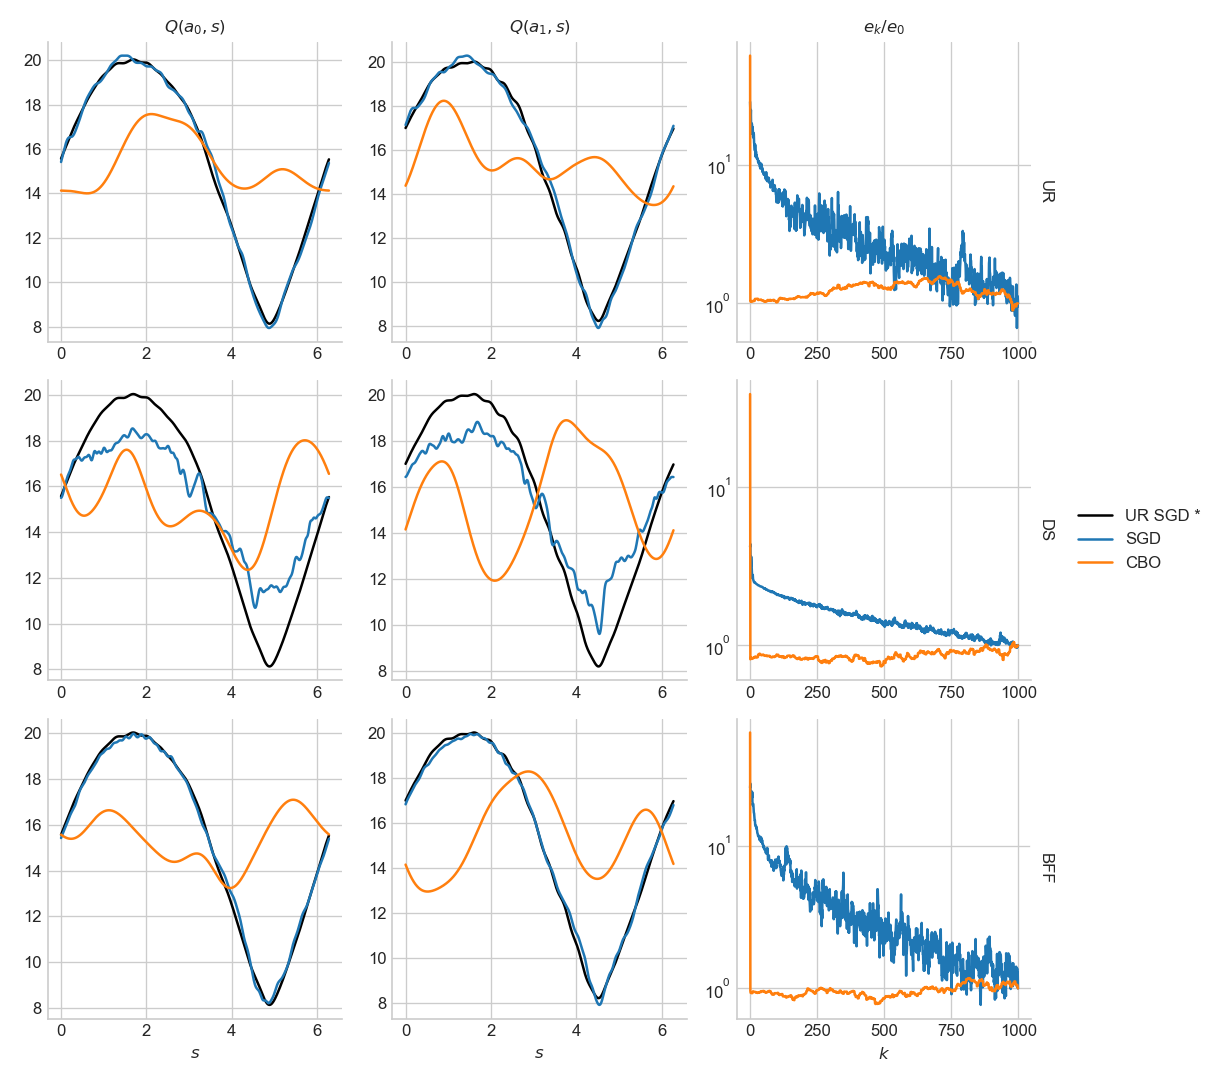
\includegraphics[width=\linewidth]{../figs/Q_ctrl_SGD_vs_CBO_summary_continuous_resnet.png}
      \caption{Summary}
      \label{fig:summary_cont}
    \end{subfigure}
    \begin{subfigure}{.5\textwidth}
      \centering
      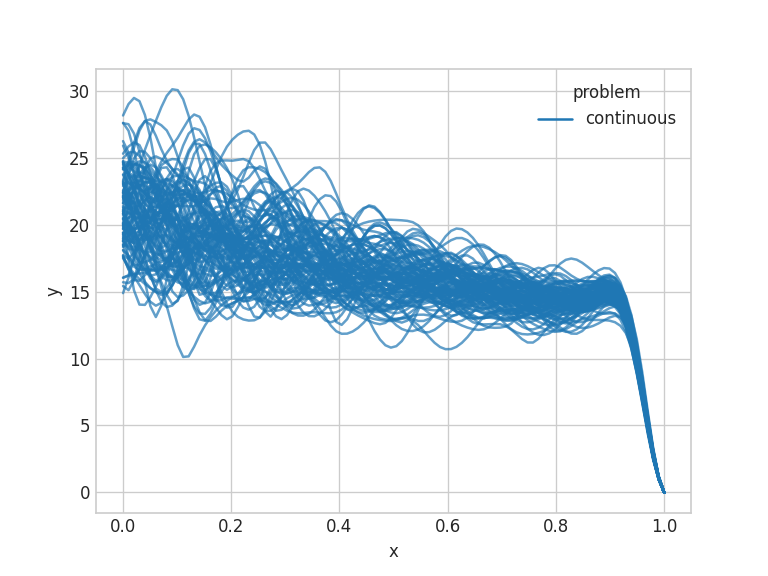
\includegraphics[width=\linewidth]{../figs/Q_ctrl_landscape_plot_continuous_resnet.png}
      \caption{Error landscape}
      \label{fig:error_landscape_cont}
    \end{subfigure}
    \caption{Continuous case}
    \label{fig:cont}
\end{figure}

\begin{figure}[H]
    \centering
    \begin{subfigure}{.9\textwidth}
      \centering
      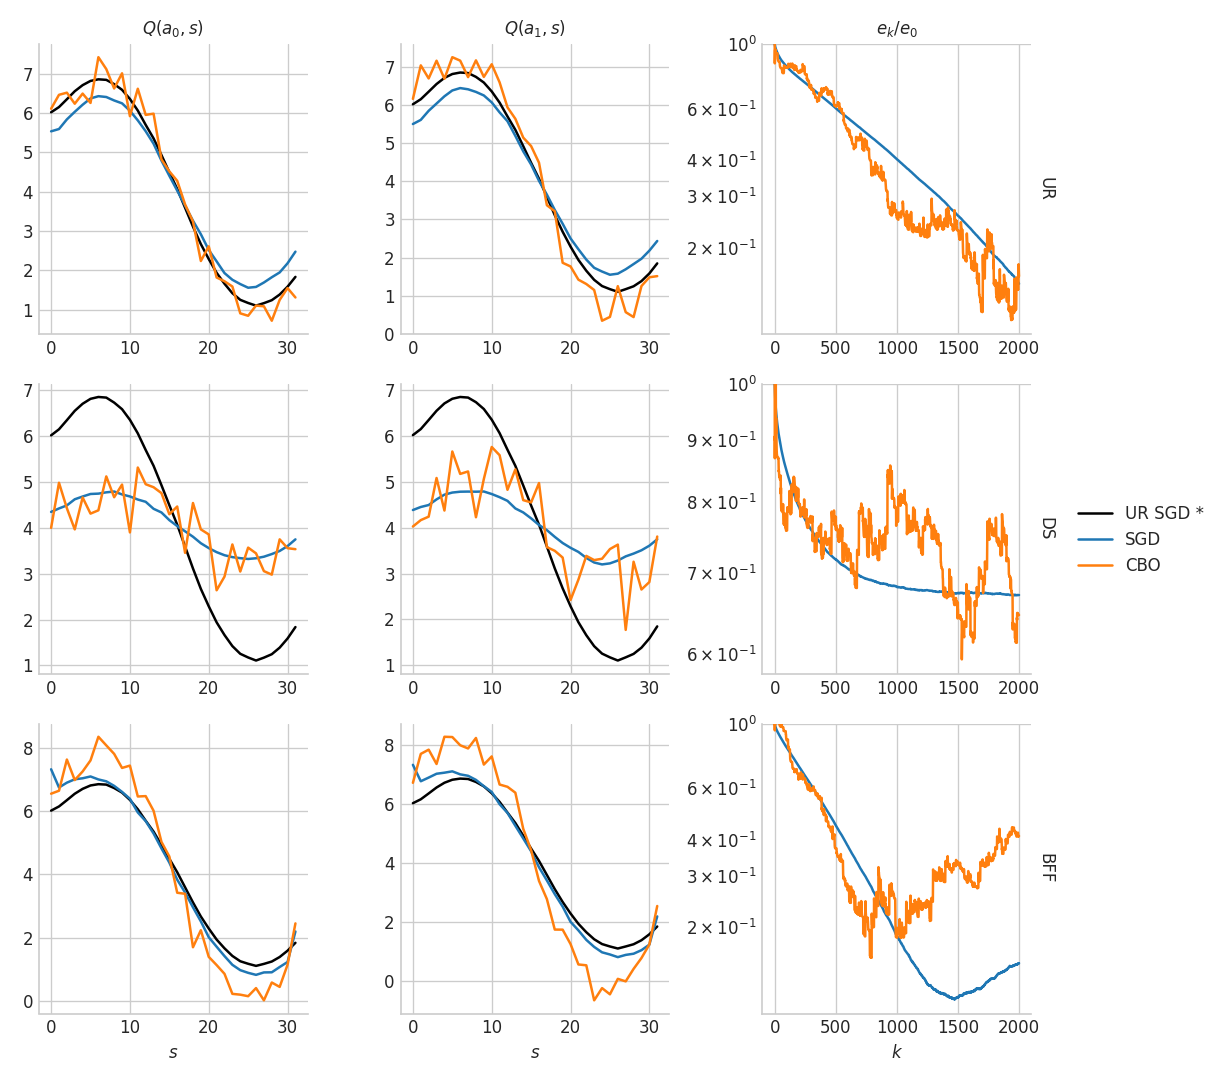
\includegraphics[width=\linewidth]{../figs/Q_ctrl_SGD_vs_CBO_summary_discrete_tabular.png}
      \caption{Summary}
      \label{fig:summary_disc}
    \end{subfigure}
    \begin{subfigure}{.5\textwidth}
      \centering
      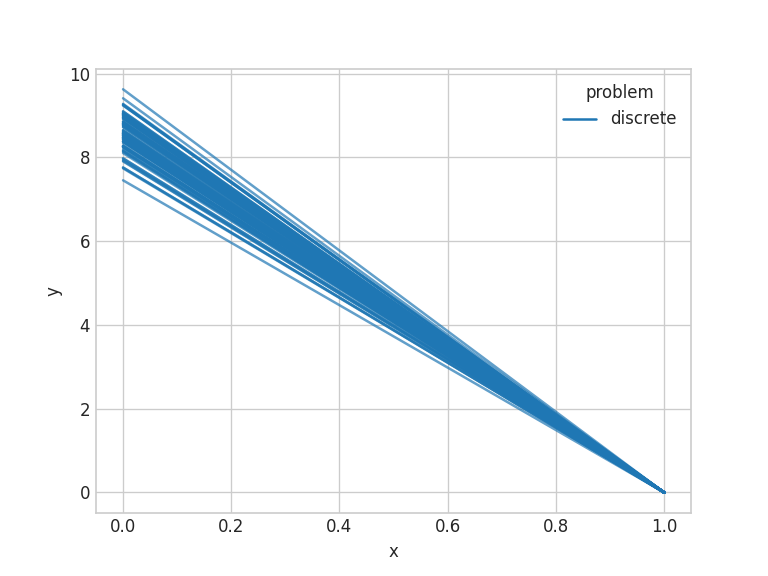
\includegraphics[width=\linewidth]{../figs/Q_ctrl_landscape_plot_discrete_tabular.png}
      \caption{Error landscape}
      \label{fig:error_landscape_disc}
    \end{subfigure}
    \caption{Discrete case}
    \label{fig:disc}
\end{figure}


\begin{table}[H]\centering
  \begin{tabular}[]{l|l}
      SGD & $\tau$\\\hline
      i & 0.08001579582322532\\
      f & 0.9835361410049764\\
      r & 0.950886309322411
  \end{tabular}
  \caption{Optimal hyperparemters for continuous case, SGD}
\end{table}

\begin{table}[H]\centering
  \begin{tabular}[]{l|lll}
      CBO & $\eta$ & $\tau$ & $\beta$\\\hline
      i & 0.27998130431694734 & 0.45180905444083275 &
      8.51669145194007\\
      f & 0.5194195083343263 & 0.4287097014952387 &
      1.7500535407136808\\
      r & 0.9698276350455655 & 0.9578569049519733 &
      1.0213109427307054
  \end{tabular}
  \caption{Optimal hyperparemters for continuous case, CBO}
\end{table}

\begin{table}[H]\centering
  \begin{tabular}[]{l|l}
  SGD & $\tau$\\\hline
  i & 4.703979337147098\\
  f & 0.654883440315296\\
  r & 0.9730502549231891
  \end{tabular}
  \caption{Optimal hyperparemters for discrete case, SGD}
\end{table}

\begin{table}[H]\centering
  \begin{tabular}[]{l|lll}
  CBO & $\eta$ & $\tau$ & $\beta$\\\hline
  i & 0.9785432879550536 & 0.893733865582011 &
  12.055703082474112\\
  f & 0.8242055859864529 & 0.3129317992204857 &
  2.6535471522264684\\
  r & 0.9827373829994701 & 0.9999130685913801 &
  1.019158705231164
  \end{tabular}
  \caption{Optimal hyperparemters for discrete case, CBO}
\end{table}



\section{Conclusion}

To summarize the results, we can say that in the Discrete + Tabular case, CBO $\gg$ SGD, BFF $>$ UR while in the Continuous + ResNet case CBO $<$ SGD and BFF $\sim$ UR.

An important note is that the differences observed above could be related to the number of variables in the hyper-parameter search (3 for SGD, 9 for CBO), as well as the complexity/convexity of the problem, ie. if we performed more trials, it might be possible for CBO $>$ SGD and BFF $>$ UR in the continuous case, although we have not observed this. This note is also based on the fact that CBO
$>$ SGD for V-eval without hyperparameter search.

\medskip

\bibliographystyle{unsrt}
\nocite{*}
\bibliography{main}

\end{document}